\section{Einführung}
\label{Einführung}
Diese Arbeit befasst sich grundlegend mit dem Fussgänger-Routing über offene Flächen im urbanen Raum und das Durchführen eines multimodalen Routings, welches das Fussgänger- und ÖV-Routing kombiniert. Im folgenden ist die Problemstellung erläutert und es wird eine Abgrenzung gemacht, was Teil dieser Arbeit ist.

\subsection{Grundlagen und Begriffe}
\label{Grundlagen und Begriffe}

Im Weiteren werden ausgewählte theoretische Grundlagen und Begriffe eingeführt, welche für das Verständnis der Arbeit von Relevanz sind. Für die nicht eingeführten Begriffe kann das Glossar und Abkürzungsverzeichnis zur Hand gezogen werden.

\subsubsection{Fläche}
\label{Fläche}

Als Fläche werden für diesen Zweck Plätze verstanden, die für Fussgänger frei begehbar sind. Flächen sind in \ac{OSM} keine eigenständige Datenelemente. Es handelt sich dabei um Polygone (sprich geschlossene Linien) oder Multipolygone (siehe \ref{Multipolygon}), welche in \ac{OSM} mit den Attributen \textit{highway=pedestrian} oder \textit{highway=footway} versehen sind. Fehlt in letzterem \textit{area=yes}, wird die geschlossene Linie als Rundweg interpretiert, über welche nicht geroutet werden soll. \cite{osm_wiki_area}

\subsubsection{nicht-motorisierter Individualverkehr}
\label{nicht-motorisierter Individualverkehr}

Zum nicht-motorisierten Individualverkehr gehören unter anderem Fussgänger, Rollstuhlfahrer und Radfahrer.

Zur besseren Lesbarkeit wird in der Arbeit nur noch von Fussgänger gesprochen. Der Fokus dieser Arbeit beschränkt sich dabei auf Fussgänger, da sich etwa für Rollstuhlfahrer und Radfahrer andere Problemstellungen auftun, welchen den Rahmen der Arbeit sprengen. 

\subsubsection{Multipolygon}
\label{Multipolygon}

Multipolygone sind in \ac{OSM} ein oder mehrere Polygone, die jeweils einen geschlossenen Pfad beschreiben. Jedes Polygon kann entweder als einen äusseren oder inneren Ring dienen. So kann ein innerer Ring eine Teilfläche eines äusseren Rings ausschneiden. Polygone in einem Multipolygon können disjunkt sein. \cite{osm_wiki_multipolygon}

\begin{figure}[th]
\centering
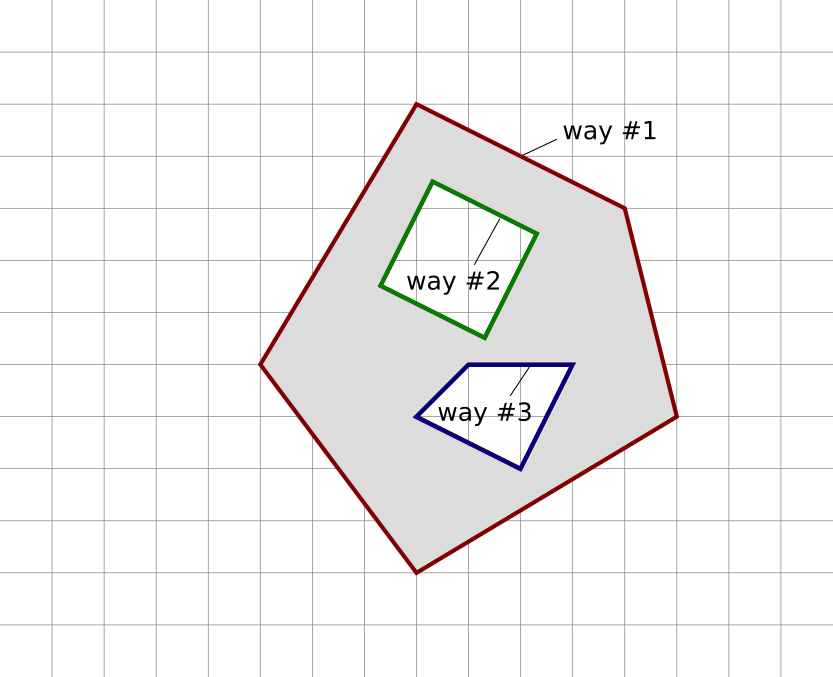
\includegraphics[width=0.5\linewidth]{technicalreport/img/multipolygon_osm_example.png}
\caption[Multipolygon OSM Example]{Beispiel eines Multipolygons in \ac{OSM} mit einem äusseren und zwei inneren Ringen. \cite{osm_wiki_multipolygon}}
\label{fig:multipolygon_osm_example}
\end{figure}

Im \ac{GIS} hingegen ist ein Multipolygon als mehrere sich nicht überschneidende Polygone definiert. Jedes Polygon wird durch ein oder mehrere geschlossene Pfade beschrieben. Dabei ist der erste Pfad der äussere Rand, alle weiteren Pfade beschreiben innere Ringe. \cite{opengis_simple_features}

\subsubsection{Hindernisse auf Flächen}
\label{Hindernisse in Flächen}

Auf Flächen können Hindernisse existieren, durch welche nicht geroutet werden darf. Dazu gehören selbstredend Gebäude und dergleichen, aber auch Barrieren, die mit  mit dem Attribut \textit{barrier=*} gekennzeichnet sind \cite{osm_wiki_barrier}, was beispielsweise eine Mauer oder Hecke beschreiben kann.

\subsubsection{ÖV-Haltestelle und Kante}
\label{ÖV-Haltestelle und Kante}
% same explanation is used in the glossary
Eine ÖV-Haltestelle kann mehrere Plattformen umfassen. Normalerweise gehören zu einer ÖV-Haltestelle zwei Plattformen, je eine in jede Fahrtrichtung. Eine dieser Plattform wird im folgenden allgemein als Kante bezeichnet. Der Unterschied ist in Abbildung \ref{fig:public_transport_stop} ersichtlich. Eine ÖV-Haltestelle muss sich dabei nicht auf zwei \glspl{Kante} beschränken. Betrachtet man den Bahnhof Stadelhofen in Zürich, Schweiz, sieht man, dass weit mehr als zwei Kanten zu einer ÖV-Haltestelle gehören können.

\begin{figure}[ht]
\centering
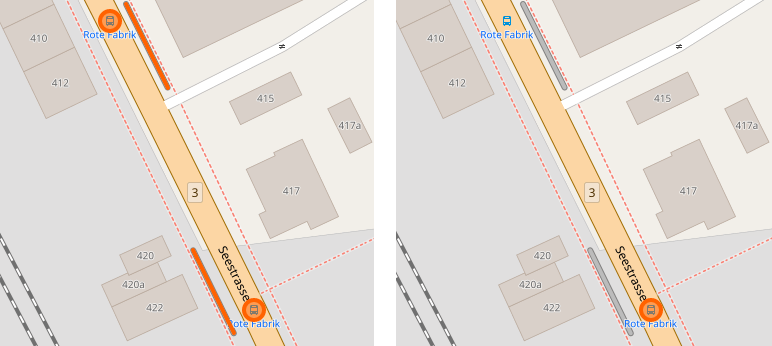
\includegraphics[width=0.7\linewidth]{technicalreport/img/public_transport_stop}
\caption[Unterschied ÖV-Haltestelle und Kante]{links: ÖV-Haltestelle; rechts: eine spezifische Kante}
\label{fig:public_transport_stop}
\end{figure}


\subsection{Problemstellung und Vision}
\label{Problemstellung und Vision}
Die heute gängigen \glspl{Routing-Engine} können effizient über Graph-Kanten und Knoten routen, um so den schnellstmöglichen Weg finden zu können. Diese wurden stetig für den motorisierten Individualverkehr optimiert, da sich diese unter anderem an vorgegebene Regeln halten und bisher einen grösseren Markt geboten haben. Bei Fussgänger ist das nicht immer der Fall. In den folgenden Unterkapiteln werden einige Probleme erläutert, welche immer noch Praxis für Fussgänger sind.

\subsubsection{Routing über offene Flächen}
\label{problem:Routing über offene Flächen}
Wie in der Abbildung \ref{fig:helvetiaplatz_graphhopper} erkennbar is, routet die Routing-Engine GraphHopper \cite{graphhopper} den Graph-Kanten nach um den Platz herum. Dies ist ein natürliches Verhalten für den motorisierten Individualverkehr. Ein Fussgänger hingegen nimmt den direkten Weg über Flächen. Oft handelt es sich dabei nicht nur um eine leere Fläche, sondern es sind Hindernisse wie Brunnen, Kunstwerke, WCs, etc. darauf stationiert, um welche auf eine natürliche Weise geroutet werden muss. Eine Route, welche direkt auf das Hindernis zusteuert, um dieses dann zu umlaufen, ist zwar ein Fortschritt zur aktuellen Lösung, entspricht aber kaum einem normalen Fussgänger-Verhalten. 

\begin{figure}[ht]
	\centering
	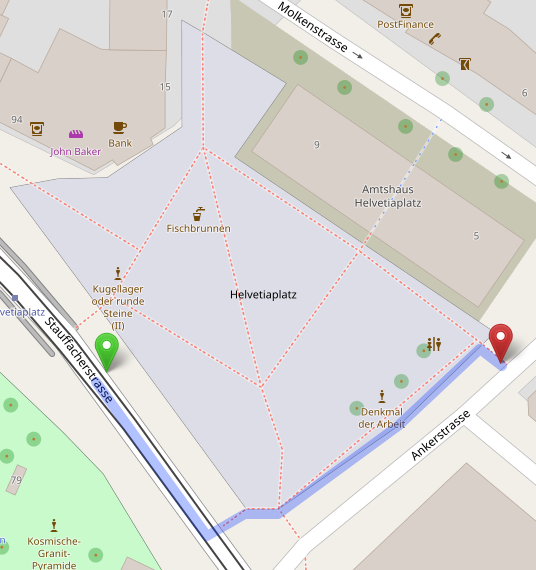
\includegraphics[width=0.5\linewidth]{technicalreport/img/helvetiaplatz_graphhopper}
	\caption[Fussgänger-Routing]{Fussgänger-Routing mit GraphHopper \cite{graphhopper} über den Helvetiaplatz, Zürich, Schweiz; Screenshot von openstreetmap.org aufgenommen am 08.10.2017}
	\label{fig:helvetiaplatz_graphhopper}
\end{figure}

\subsubsection{eingezeichnete Fussgängerrouten über offene Flächen}
\label{problem:eingezeichnete Fussgängerrouten über offene Flächen}
Wenn man die gleiche Abbildung \ref{fig:helvetiaplatz_graphhopper} nochmals betrachtet, sieht man, dass Mapper bereits einige Fusswege auf dem Platz eingezeichnet haben, um dem Routing-Problem über offene Flächen entgegen zu steuern. Dies kann in einigen Situationen wie dem Helvetiaplatz kontraproduktiv, aber in anderen wieder von Vorteil sein. Betrachtet man beispielsweise den Central Park in New York in Abbildung \ref{fig:central_park}, macht es Sinn, dass das Routing den vorgegebenen Wegen folgt. Eine Wiese gilt als offene Fläche, eignet sich aber nicht immer als vorteilhafter Bewegungsuntergrund. 

\begin{figure}[ht]
\centering
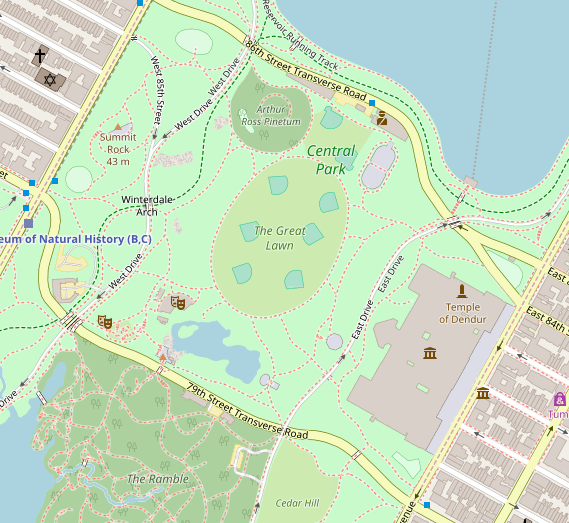
\includegraphics[width=0.5\linewidth]{technicalreport/img/central_park}
\caption[eingezeichnete Fussgänger-Routen]{Eingezeichnete Fussgänger-Routen auf dem Central Park, New York City, USA; Screenshot von openstreetmap.org aufgenommen am 08.10.2017}
\label{fig:central_park}
\end{figure}

\subsubsection{topologisch nicht verbundene Wege}
\label{problem:topologisch nicht verbundene Wege}

\begin{figure}[ht]
\centering
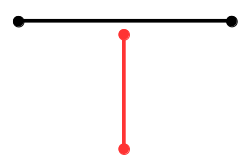
\includegraphics[width=0.5\linewidth]{technicalreport/img/topologisch_nicht_verbundener_graph}
\caption[topologisch nicht verbundener Graph]{topologisch nicht verbundener Graph}
\label{fig:topologisch_nicht_verbundener_graph}
\end{figure}

In Abbildung \ref{fig:topologisch_nicht_verbundener_graph} ist ein topologisch nicht verbundener Graph zu sehen. In \ac{OSM} kann es vorkommen, dass solche Wege auf eine offene Fläche treffen, mit dieser aber nicht topologisch verbunden sind. Eine \gls{Routing-Engine} muss in der Lage sein, dies zu erkennen und aufzuräumen, so dass vom auftreffenden Weg über die offene Fläche geroutet werden kann.

\subsubsection{Routing über über weitere Arten von offenen Flächen (Berge, Strände)}
\label{problem:Routing über über weitere Arten von offenen Flächen (Berge, Strände)}
Berge und Strände sind bekanntermassen schwieriger zu überqueren als normale Plätze. Sei dies aufgrund der zurückzulegenden Höhendifferenz oder der Unterlage, welche das Fortbewegen einschränkt. Zusätzlich zum Problem \ref{problem:Routing über offene Flächen} kommt hier dazu, dass das Umlaufen dieser offenen Flächen (Berge, Strände) in manchen Situationen effizienter sein kann als das Überqueren.

\subsubsection{Datenaufbereitung für das Fussgänger-Routing über Strassen}
\label{problem:Datenaufbereitung für das Fussgänger-Routing über Strassen}
Beim Fussgänger-Routing über Strassen ergeben sich andere Anforderungen als beim Routing für den motorisierten Individualverkehr. So müssen etwa Bürgersteige und Fussgänger-Streifen beachtet werden, um zu entscheiden, ob eine Strasse für Fussgänger begehbar ist.

\subsubsection{Start-/Endpunkt auf der Fläche}
\label{problem:Start-/Endpunkt auf der Fläche}
Beginnt das Routing oder ist der Zielort auf einer Fläche, so ziehen die aktuellen \glspl{Routing-Engine}, falls keine Wege wie in \ref{problem:eingezeichnete Fussgängerrouten über offene Flächen} beschrieben eingezeichnet sind, eine Mittelsenkrechte zur nächsten Polygonkante der Fläche und routen von dort weiter. Dies ist gut auf dem Sechseläutenplatz in Abbildung \ref{fig:start_endpoint_on_area} sichtbar. Falls bereits Wege auf der Fläche eingezeichnet sind, wird über diese geroutet.

\begin{figure}[ht]
    \centering
    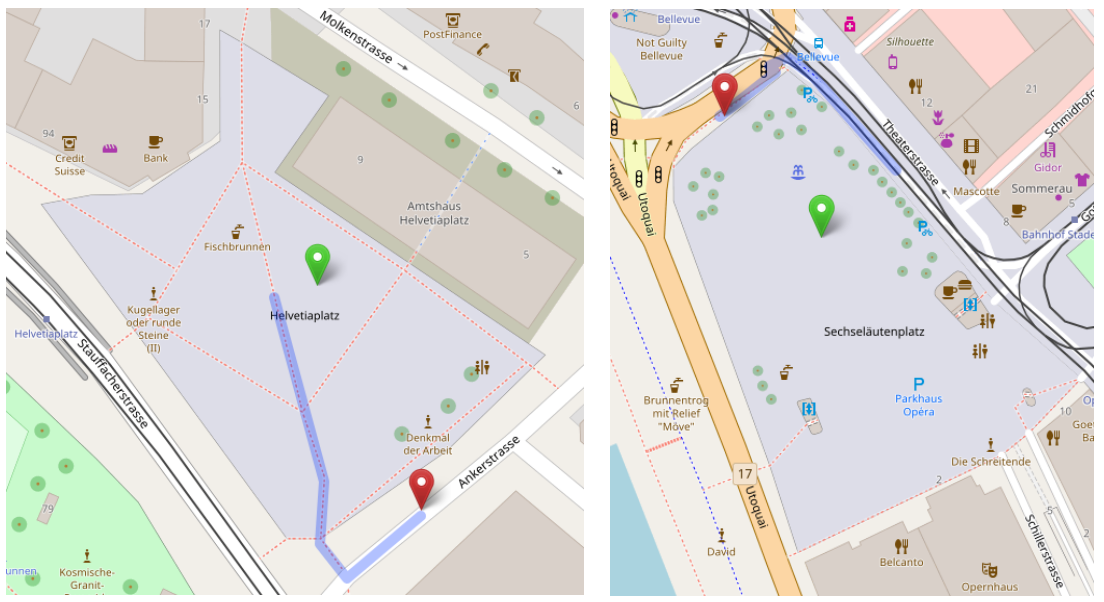
\includegraphics[width=1\linewidth]{technicalreport/img/start_endpoint_on_area}
    \caption[Fussgänger-Routing mit Startpunkt auf der Fläche]{Fussgänger-Routing mit GraphHopper über den Helvetiaplatz (links) und Sechseläutenplatz (rechts), Zürich, Schweiz mit Startpunkt auf der Fläche; Screenshot von openstreetmap.org aufgenommen am 14.10.2017}
    \label{fig:start_endpoint_on_area}
\end{figure}

\subsubsection{Routing bei zwei benachbarten Flächen}
\label{problem:Routing bei zwei benachbarten Flächen}
Es kann vorkommen, dass zwei Flächen unmittelbar nebeneinander liegen. Dies ist beim Bundesplatz in Bern, Schweiz der Fall, welcher direkt an den Bärenplatz grenzt. Dies ist in Abbildung \ref{fig:bundesplatz_baerenplatz} sichtbar. Das erschwert das Routing über Flächen, da nicht direkt \glspl{Einstiegspunkt} eines Polygons genutzt werden können.

\begin{figure}[ht]
\centering
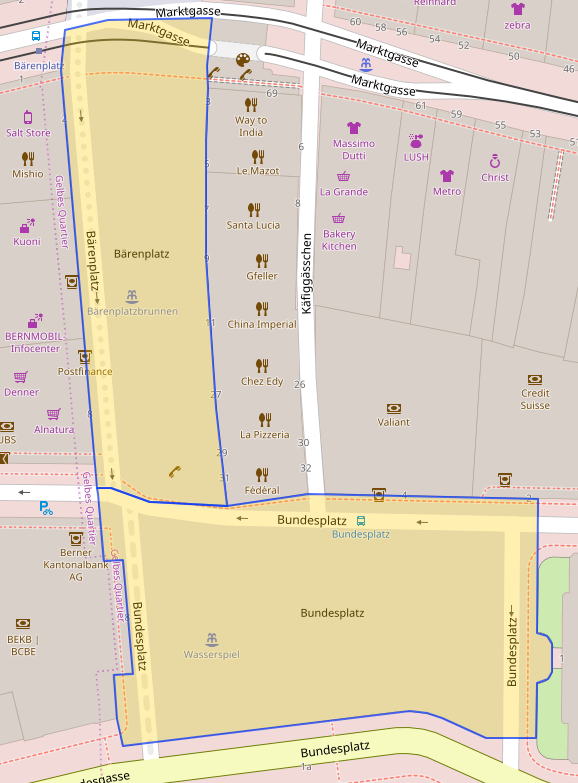
\includegraphics[width=0.5\linewidth]{technicalreport/img/bundesplatz_baerenplatz}
\caption[Zwei benachbarte Flächen]{Zwei benachbarte Flächen (Bundesplatz, Bärenplatz) in Bern, Schweiz; Screenshot von overpass-turbo.eu aufgenommen am 18.10.2017}
\label{fig:bundesplatz_baerenplatz}
\end{figure}

\subsubsection{mehrere Kanten mit dem gleichen Namen}
\label{problem:mehrere Kanten mit dem gleichen Namen}
In den meisten Fällen gibt es an einem Standort mit einer ÖV-Haltestelle zwei \glspl{Kante} mit dem gleichen Namen, je eine für die jeweilige Fahrtrichtung. In manchen Fällen ist es so, dass diese Kanten ein Stück voneinander entfernt liegen. Es muss entschieden werden, zu welcher Kante geroutet werden soll.
	
\subsection{Ziele und Unterziele}
\label{Ziele und Unterziele}

\subsubsection{Routing über offene Flächen}
\label{target:Routing über offene Flächen}
Das Problem wie in \ref{problem:Routing über offene Flächen} beschrieben wurde bereits in einigen Arbeiten aufgegriffen \cite{graser_visibility_graph} \cite{dzafic_spider_web_graph}. Diese beiden Ansätze (Visibility-Graph und SpiderWeb-Graph) werden analysiert, dazu Tests in \gls{QGIS} implementiert und mit Probanden getestet. Ziel ist es, die optimale Variante zu eruieren, um über offene Flächen routen zu können. Diese Variante soll so aufbereitet werden, dass eine \ac{OSM}-Datei so verarbeitet werden kann, dass danach eine Routing-Engine auf diesen Daten operieren kann.

\subsubsection{Routing-Engine evaluieren}
\label{target:Routing-Enginge evaluieren}
Die "grösseren" \glspl{Routing-Engine} sollen analysiert und es soll festgehalten werden, welche sich für den Hauptzweck dieser Arbeit am besten eignet. Zusätzlich wird geprüft, wie die verarbeitenden Daten aus \ref{target:Routing über offene Flächen} in die bestehenden Routing-Engines eingehängt werden können.

\subsubsection{eingezeichnete Fussgängerrouten über offene Flächen}
\label{target:eingezeichnete Fussgängerrouten über offene Flächen}
Im Kontext dieser Arbeit werden die Pfade beibehalten und keine weiteren Abklärungen bezüglich dieser Fragestellung unternommen. Im Hinblick auf eine Folgearbeit wäre es von Interesse zu wissen, in welchen Situation man sich auf vorhandene Wege über offene Flächen verlassen kann (wie in Abbildung \ref{fig:central_park}) und wann sie zu ignorieren sind. Es gilt zu prüfen, ob diese Abgrenzung mit den gegebenen Informationen überhaupt möglich ist. 

\subsubsection{topologisch nicht verbundene Wege}
\label{target:topologisch nicht verbundene Wege}
Dieses Problem ist der Vollständigkeit halber aufgeführt, wird in dieser Arbeit aber nicht weiter verfolgt.

\subsubsection{Routing über über weitere Arten von offenen Flächen (Berge, Strände)}
\label{target:Routing über über weitere Arten von offenen Flächen (Berge, Strände)}
Im Kontext dieser Arbeit wird kurz ein theoretischer Ansatz aufgezeigt, wie man mit einem kostenbasierten Graphen den Eigenschaften diesen Unterflächen gerecht werden könnte.

\subsubsection{Datenaufbereitung für das Fussgänger-Routing über Strassen}
\label{target:Datenaufbereitung für das Fussgänger-Routing über Strassen}

In dieser Arbeit wird der aktuelle Stand und die Herausforderungen für die Datenaufbereitung für allgemeines Fussgänger-Routings aufgezeigt. Für das Routing über offene Flächen sind diese Probleme allerdings nicht weiter relevant. Wir gehen davon aus, dass die verwendeten \glspl{Routing-Engine} ein genügend gutes Verhalten für Fussgänger-Routing über Strassen aufzeigen.

\subsubsection{Start-/Endpunkt auf der Fläche}
\label{target:Start-/Endpunkt auf der Fläche}
Der Fussgänger-Routing kann von einem beliebigen Startpunkt aus gestartet werden. Somit soll es möglich sein, dass das Routing auf einer Fläche beginnen kann und man nicht wie in \ref{problem:Start-/Endpunkt auf der Fläche} beschrieben zur nächstgelegenen Polygonkante geroutet wird. Es soll geklärt werden, ob die Vorverarbeitung der Flächen, wie es in \ref{target:Routing über offene Flächen} vorgesehen ist, ausreicht, oder ob zu einem späteren Zeitpunkt ein Echtzeit-Verarbeitung der Fläche vom aktuellen Standort aus in Betracht gezogen werden muss.

\subsubsection{Routing bei zwei benachbarten Flächen}
\label{target:Routing bei zwei benachbarten Flächen}

Es soll geprüft werden, wie Fussgänger-Flächen bearbeitet werden können, die direkt benachbart sind. Wenn die beiden Flächen unabhängig voneinander verarbeitet werden, gibt es unter Umständen eine Polygonkante, die von einem Fussgänger problemlos übergangen werden könnte, logisch aber als eine Abgrenzung interpretiert wird, die in der Route nicht überquert wird.

\subsubsection{nächste ÖV-Haltestellen finden}
\label{target:nächste ÖV-Haltestellen finden}
Ein weiterer Fokus der Arbeit liegt auf dem Finden und Erreichen der nächsten ÖV-Haltestelle, von welcher ein ÖV-Routing durchgeführt werden kann. So soll eruiert werden, wie von einem bestehenden Startpunkt aus die nächsten ÖV-Haltestellen identifiziert werden können, um diese an search.ch für das weitere ÖV-Routing zu übergeben.

\subsubsection{mehrere Kanten mit dem gleichen Namen}
\label{target:mehrere Kanten mit dem gleichen Namen}
Wurde die nächste ÖV-Haltestelle wie in \ref{target:nächste ÖV-Haltestellen finden} beschrieben eruiert, so gilt es, zur \gls{Kante} in die richtige Fahrtrichtung zu routen.

\subsubsection{Prototyp und Deliverables}
\label{target:Prototyp und Deliverables}
Das Resultat besteht aus zwei Teilen. Einerseits wird es möglich sein, \ac{OSM}-Daten vorzuverarbeiten, welche an eine \gls{Routing-Engine} übergeben werden können, um das Fussgänger-Routing im urbanen Raum sicherzustellen. Andererseits wird ein Backend entwickelt, welches ein multimodales Routing, sprich Fussgänger- in Kombination mit einem ÖV-Routing anbietet. In einem weiteren Schritt wird die Vorverarbeitung und das multimodale Routing in einem QGIS-Plugin sichtbar gemacht. Die detaillierten Anforderungen sind im Teil \ref{chap:SW-Projektdokumentation} Kapitel \ref{sec:Anforderungsspezifikation} beschrieben.
	
\subsection{Rahmenbedingungen, Umfeld, Definitionen und Abgrenzungen}
\label{Rahmenbedingungen, Umfeld, Definitionen, Abgrenzungen}
Die Arbeit befasst sich mit Flächen im urbanen Raum. Berge, Strände, Parks, etc. werden bewusst ausgeklammert, um nicht den Rahmen der Arbeit zu sprengen. Voraussetzung ist, dass Python als Programmiersprache verwendet wird und \ac{OSM}-Daten \cite{osm_data_switzerland} verarbeitet werden.

Als Drittsysteme sind das \ac{API} von search.ch \cite{search_ch_route_api} für das ÖV-Routing, Overpass \cite{wiki:overpass} für das Extrahieren von spezifischen \ac{OSM}-Daten und Nominatim \cite{nominatim_osm} für das \gls{Geocoding} zu gebrauchen.

Die Backend-Komponente sollen als Docker-Container für eine einfache Portierung und Deployment verfügbar sein. Die Funktionalität der Komponenten wird kontinuierlich mit Continuous Integration sichergestellt.

\subsection{Vorgehen und Aufbau der Arbeit}
\label{Vorgehen und Aufbau der Arbeit}
Die Studienarbeit nimmt sich zu erst dem Problem des Fussgänger-Routing über Flächen im urbanen Raum an. Es wird geklärt, wie der Stand der Technik ist und welche Vorarbeiten und Lösungen in diesem Bereich existieren. Bestehende Lösungsvorschläge werden in Python implementiert und in \gls{QGIS} getestet, um so die bestmögliche Variante zu eruieren. Sobald die optimale Lösungsvarianten identifiziert sind, muss geklärt werden, wie die Vorverarbeitung der Daten (beispielsweise das Einzeichnen von möglichen Routen über Flächen) an eine bestehende Routing-Engine übergeben werden kann. Damit dies möglich ist, ist zu prüfen, welche Routing-Engine die Anforderungen bestmöglich abdeckt.

In einem weiteren Schritt soll ermittelt werden, wie die nächsten ÖV-Haltestellen eruiert werden können, um diese Punkte an das \ac{API} von search.ch \cite{search_ch_route_api} übergeben zu können. Aufgabe von search.ch ist es, für einen Start und eine Destination die ÖV-Route zu genieren. So kann der schnellstmögliche Weg von einem beliebigen Punkt an ein beliebiges Ziel in Kombination mit Fussweg und öffentlichem Verkehr ermittelt werden.

Die vorhin aufgeführten Aspekte werden im Teil \ref{chap:Technischer Bericht} behandelt.

In einem zweiten Teil werden die im Teil \ref{chap:Technischer Bericht} erarbeiteten Artefakte in einem Prototyp als QGIS-Plugin zusammengeführt. Im QGIS-Plugin wird ein multimodales Routing visuell dargestellt. So ist ein optimiertes Fussgänger-Routing in Kombination mit dem öffentlichen Verkehr möglich. Dazu müssen \ac{OSM}-Daten für das Fussgänger-Routing über offene Flächen in urbanen Raum aufbereitet werden können und das multimodale Routing als Backend verfügbar sein.

Die Implementation wird im Teil \ref{chap:SW-Projektdokumentation} beschrieben.
